\documentclass[titlepage]{scrartcl}
\usepackage{enumitem}
\usepackage[british]{babel}
\usepackage[style=apa, backend=biber]{biblatex}
\DeclareLanguageMapping{british}{british-apa}
\usepackage{url}
\usepackage{float}
\usepackage{caption}
\restylefloat{table}
\usepackage{perpage}
\MakePerPage{footnote}
\usepackage{abstract}
\usepackage{graphicx}
% Create hyperlinks in bibliography
\usepackage{hyperref}
\usepackage{amsmath}

\usepackage[T1]{fontenc}
\usepackage[utf8]{inputenc}
\usepackage{blindtext}
\setkomafont{disposition}{\normalfont\bfseries}

\graphicspath{
    {./resources/},
}
\addbibresource{~/Documents/library.bib}


\newsavebox{\abstractbox}
\renewenvironment{abstract}
  {\begin{lrbox}{0}\begin{minipage}{\textwidth}
   \begin{center}\normalfont\sectfont\abstractname\end{center}\quotation}
  {\endquotation\end{minipage}\end{lrbox}%
   \global\setbox\abstractbox=\box0 }

\usepackage{etoolbox}
\makeatletter
\expandafter\patchcmd\csname\string\maketitle\endcsname
  {\vskip\z@\@plus3fill}
  {\vskip\z@\@plus2fill\box\abstractbox\vskip\z@\@plus1fill}
  {}{}
\makeatother

\DeclareCiteCommand{\citeyearpar}
    {}
    {\mkbibparens{\bibhyperref{\printdate}}}
    {\multicitedelim}
    {}

% MATLAB Code block stuff...
\usepackage{color}
\usepackage{listings}

\definecolor{dkgreen}{rgb}{0,0.6,0}
\definecolor{gray}{rgb}{0.5,0.5,0.5}

\newcommand{\code}[1]{\texttt{#1}}

\lstset{language=Matlab,
    keywords={break,case,catch,continue,else,elseif,end,for,function,
        global,if,otherwise,persistent,return,switch,try,while},
    basicstyle=\ttfamily,
    keywordstyle=\color{blue},
    commentstyle=\color{gray},
    stringstyle=\color{dkgreen},
    numbers=left,
    numberstyle=\tiny\color{gray},
    stepnumber=1,
    numbersep=10pt,
    backgroundcolor=\color{white},
    tabsize=4,
    showspaces=false,
    showstringspaces=false
    frame=single,
    breaklines=true,
    %postbreak=\raisebox{0ex}[0ex][0ex]{\ensuremath{\color{red}\hookrightarrow\space}}
}

\begin{document}
\title{ECS708P/U - Machine Learning}
\subtitle{\LARGE{Assignment 1 Report\\Linear, Logistic Regression}}
\author{Sam Perry - EC16039}

\maketitle

\section{Linear Regression}
\subsection{Modify the function \code{calculate\_hypothesis.m} to return the predicted value for a single specified training example}
\begin{lstlisting}
function hypothesis = calculate_hypothesis(X, theta, training_example)
    % Calculates the hypothesis for a given X, theta and specified training example
    % Get bias term
    x0 = X(training_example, 1);
    % Get first term
    x1 = X(training_example, 2);

    % Calculate output hypothesis
    hypothesis = theta(1)*x0+theta(2)*x1;
end
\end{lstlisting}\leavevmode \\

\subsection{Notice that the hypothesis function is not being used in the
\code{gradient\_descent} function. Modify this to use the
\code{calculate\_hypothesis} function}
\begin{lstlisting}[firstnumber=27]
        ...
        for i = 1:m
            hypothesis = calculate_hypothesis(X, theta, i);
            output = y(i);
            sigma = sigma + (hypothesis - output);
        end

        theta_0 = theta_0 - ((alpha * 1.0) / m) * sigma;

        sigma = 0.0;

        for i = 1:m
            hypothesis = calculate_hypothesis(X, theta, i);
            output = y(i);
            sigma = sigma + (hypothesis - output) * X(i, 2);
        end
        ...
\end{lstlisting}\leavevmode \\
 
\subsection{Observe what happens when you use a very high or very low learning
rate}
When a very low alpha value ($\alpha=0.0001$) is used, the reduction in cost
per iteration is not sufficient to generate an accurate function. Many more
iterations would be needed to produce a value of $\theta$ close to the desired
local minima. This is illustrated in figures~\ref{LowLearnFunc} and
~\ref{LowLearnCost}.\\

A high value for alpha ($\alpha=1.0$) will result in large shifts in the
function over each iteration. This causes $\theta$ to diverge in the gradient
descent algorithm, increasing between positive and negative values further away
from the minima on each iteration. The final result of this can be seen in
figure~\ref{HighLearnFunc}. The exponential increase in cost causes only the
final increase to be clear through figure~\ref{HighLearnCost}.

\begin{figure}
    \caption{Hypothesis Function ($\alpha=0.0001$)}
    \makebox[\textwidth]{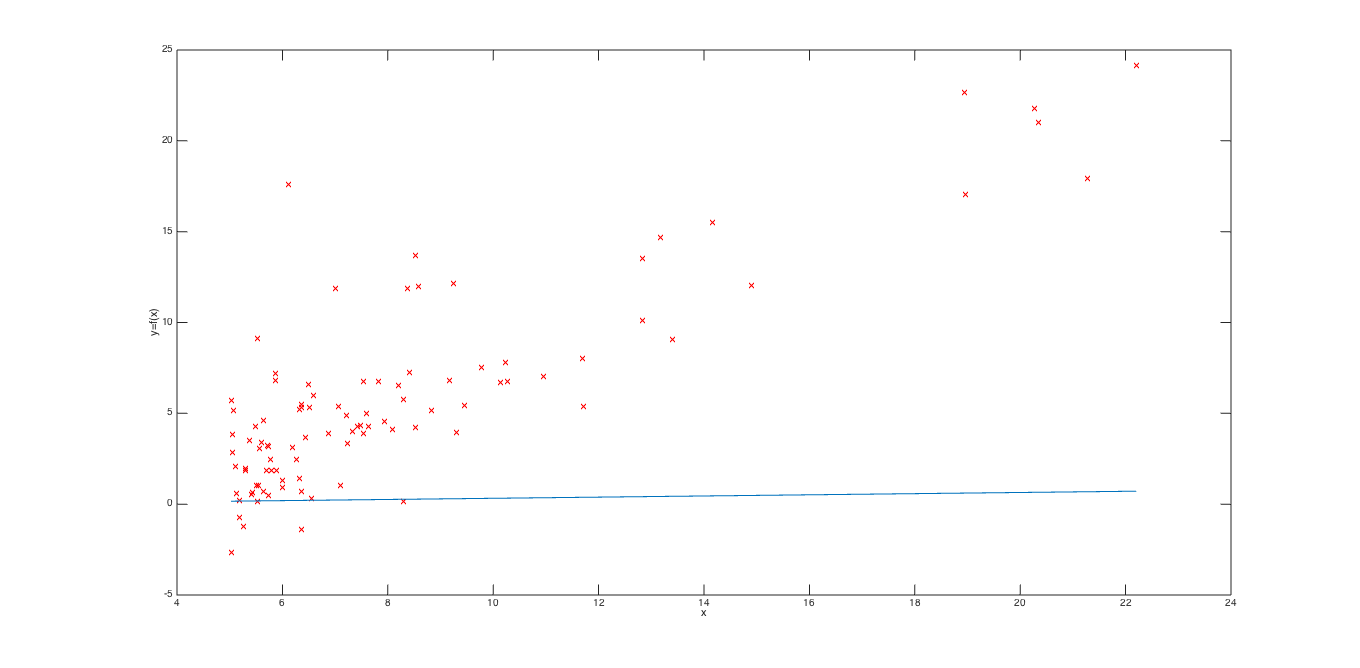
\includegraphics[width=1\textwidth]{LowLearningRateFunc}}
    \label{LowLearnFunc}
    \caption{Cost Function ($\alpha=0.0001$)}
    \makebox[\textwidth]{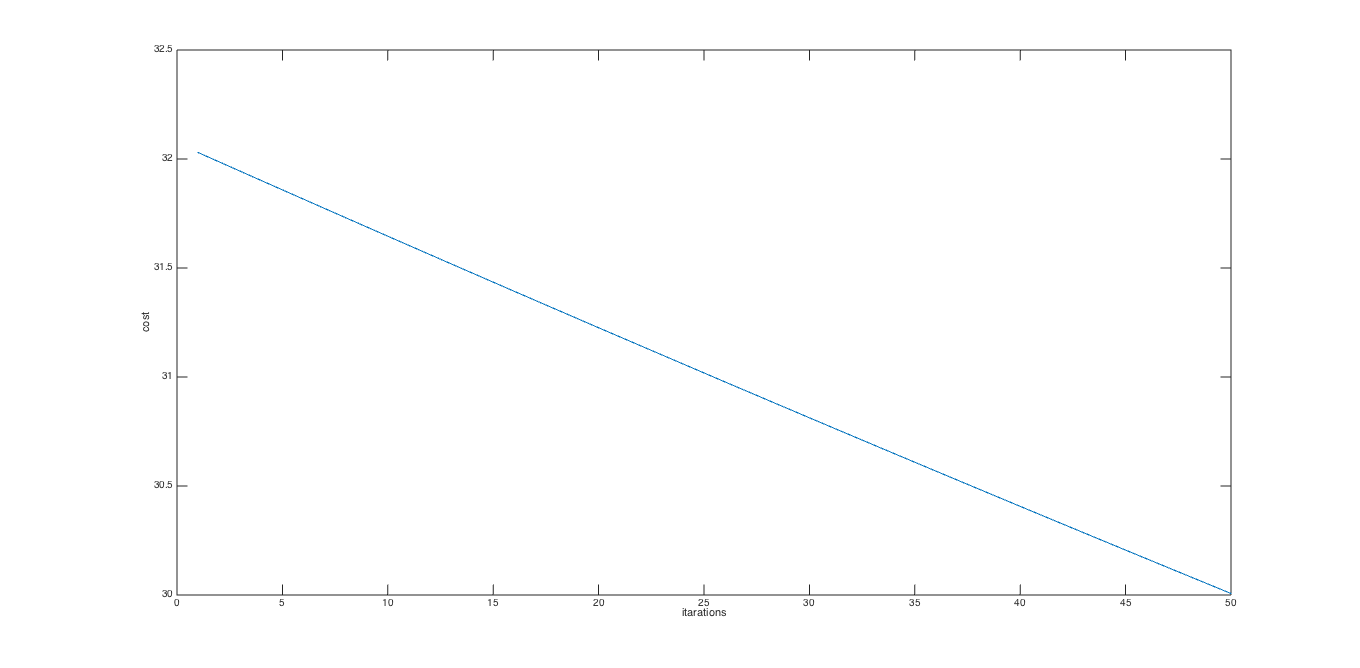
\includegraphics[width=1\textwidth]{LowLearningRateCost}}
    \label{LowLearnCost}
\end{figure}

\begin{figure}
    \caption{Hypothesis Function ($\alpha=1.0$)}
    \makebox[\textwidth]{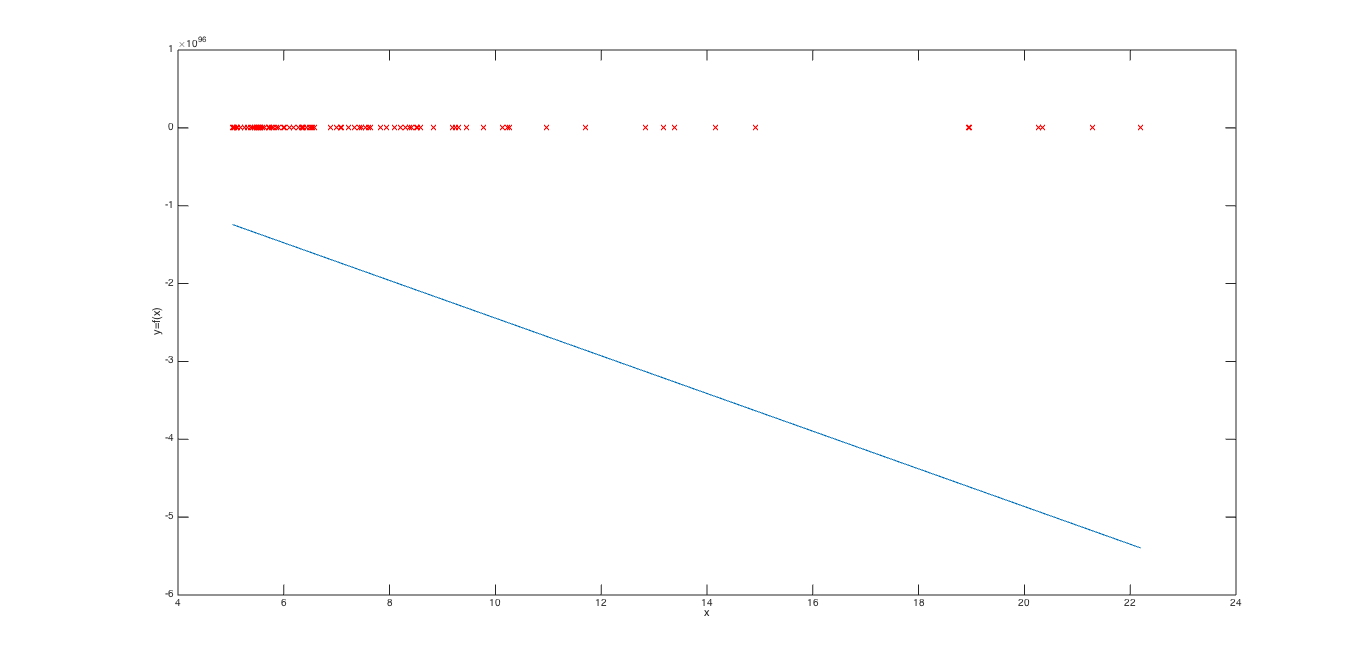
\includegraphics[width=1\textwidth]{HighLearningRateFunc}}
    \label{HighLearnFunc}
    \caption{Cost Function ($\alpha=1.0$)}
    \makebox[\textwidth]{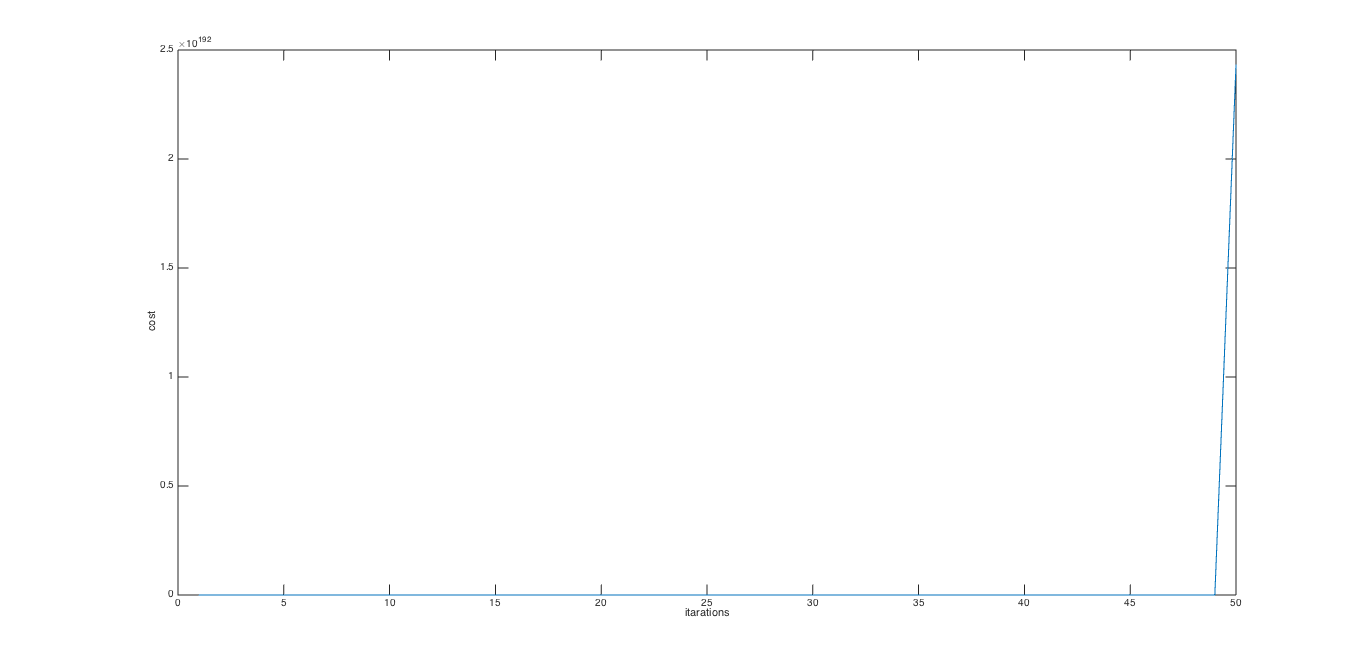
\includegraphics[width=1\textwidth]{HighLearningRateCost}}
    \label{HighLearnCost}
\end{figure}

\subsection{Modify the functions \code{calculate\_hypothesis} and
    \code{gradient\_descent} to support the new hypothesis. This should be
    sufficiently general so that we can have any number of extra variables.}
\begin{lstlisting}
function hypothesis = calculate_hypothesis(X, theta, training_example)
    % CALCULATE_HYPOTHESIS This calculates the hypothesis for a given X,
    % theta and specified training example
    x = X(training_example, 1:length(theta));

    % Calculate the hypothesis as the sum of x values multiplied by there
    % relevant theta values.
    hypothesis = sum(x.*theta);
end
\end{lstlisting}\leavevmode \\

\subsection{Print the theta values found at the end of the optimization. Does anything surprise you?}
The final values for $\theta$ were:\\
$\theta = \big[ 340412.659574468, 110631.050278846, -6649.4742708198 \big]$\\
          
It is suprising that the $\theta$ value relating to the number of rooms is
negative, suggesting that a house of a certain size tends to be worth less if
it has a high quantity of rooms when compared to a house of similar size that
has less.

\subsection{How much does you algorithm predict that a house with 1650 sq. ft.
and 3 bedrooms cost? How about 3000 sq. ft. and 4 bedrooms?}

The formula:
$$h_\theta(x)=\theta_0x_0+\theta_1x_1+\theta_2x_2$$

was applied to the new values (pre-normalized) $x_1=1650, x_2=3$ using the calculated
values for $\theta$. From this, a predicted house price of \$293,083 was generated
(rounded to the nearest \$).\\
For values $x_1=3000, x_2=4$ a price of \$472,277 was predicted.

\subsection{modify \code{gradient\_descent} to use the
\code{compute\_cost\_regularised} method instead of \code{computer\_cost}}

\begin{lstlisting}
function theta = gradient_descent(X, y, theta, alpha, iterations, l, do_plot)
...
\end{lstlisting}

\begin{lstlisting}[firstnumber=40]
...
%update cost_vector
cost_vector = [cost_vector; compute_cost_regularised(X, y, theta, l)];
...
\end{lstlisting}\leavevmode \\

\subsection{Modify \code{gradient\_descent} to incorporate the new cost function}

\begin{lstlisting}[firstnumber=23]
...
for ind = 1:length(theta_temp)
    %update theta(1) and store in temporary variable theta_0
    sigma = 0.0;

    for i = 1:m
        hypothesis = calculate_hypothesis(X, theta, i);
        output = y(i);
        sigma = sigma + (hypothesis - output) * X(i, ind);
    end

    % Apply regularization to all terms aside from the bias term.
    if ind > 1
        theta_temp(ind) = (theta_temp(ind) * (1.0-alpha*(l/m))) - ((alpha * 1.0) / m) * sigma;
    else
        theta_temp(ind) = theta_temp(ind) - ((alpha * 1.0) / m) * sigma;
    end
end
...
\end{lstlisting}\leavevmode \\


\subsection{Find the best values of $\alpha$ to use in order to optimize best}
Through trial and error, the value for alpha that best fit the data was found
to be around 1.461. Higher values than this were found to diverge. The cost and
hypothesis functions are shown in figures~\ref{PolynomialAlphaOnlyFunc}
and~\ref{PolynomialAlphaOnlyCost}.

\begin{figure}
    \caption{Hypothesis Function ($\alpha=1.461$)}
    \makebox[\textwidth]{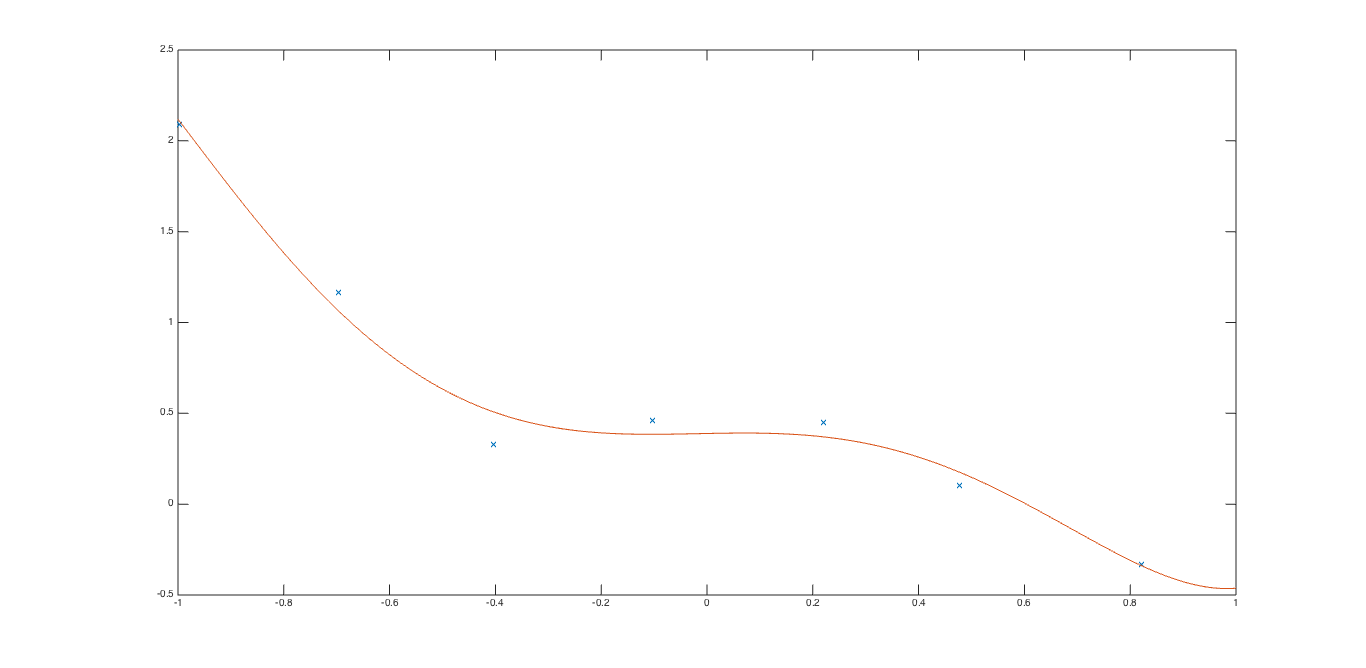
\includegraphics[width=1\textwidth]{PolynomialAlphaOnlyFunc}}
    \label{PolynomialAlphaOnlyFunc}
    \caption{Cost Function ($\alpha=1.461$)}
    \makebox[\textwidth]{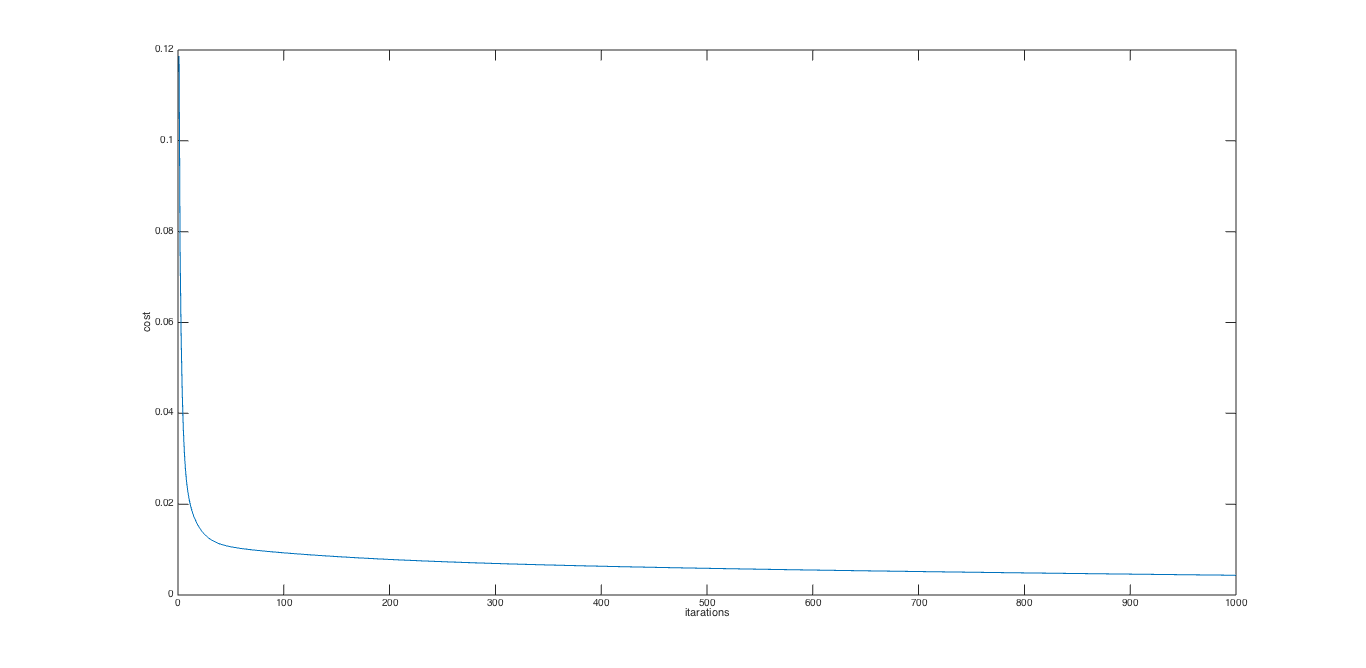
\includegraphics[width=1\textwidth]{PolynomialAlphaOnlyCost}}
    \label{PolynomialAlphaOnlyCost}
\end{figure}

\subsection{Experiment with different values of $\lambda$ and see how this affects the
    shape of the hypothesis.}
It appears that increasing value for $\lambda$ results in the flattening of the
hypothesis function. This is due to the penalisation of higher order terms in
the calculation of the hypothesis function. The results of $\alpha=1.2,
\lambda=3.0$ is shown in figure~\ref{PolynomialAlphaLambdaFunc}.

\begin{figure}
    \caption{Hypothesis Function ($\alpha=1.2, \lambda=3.0$)}
    \makebox[\textwidth]{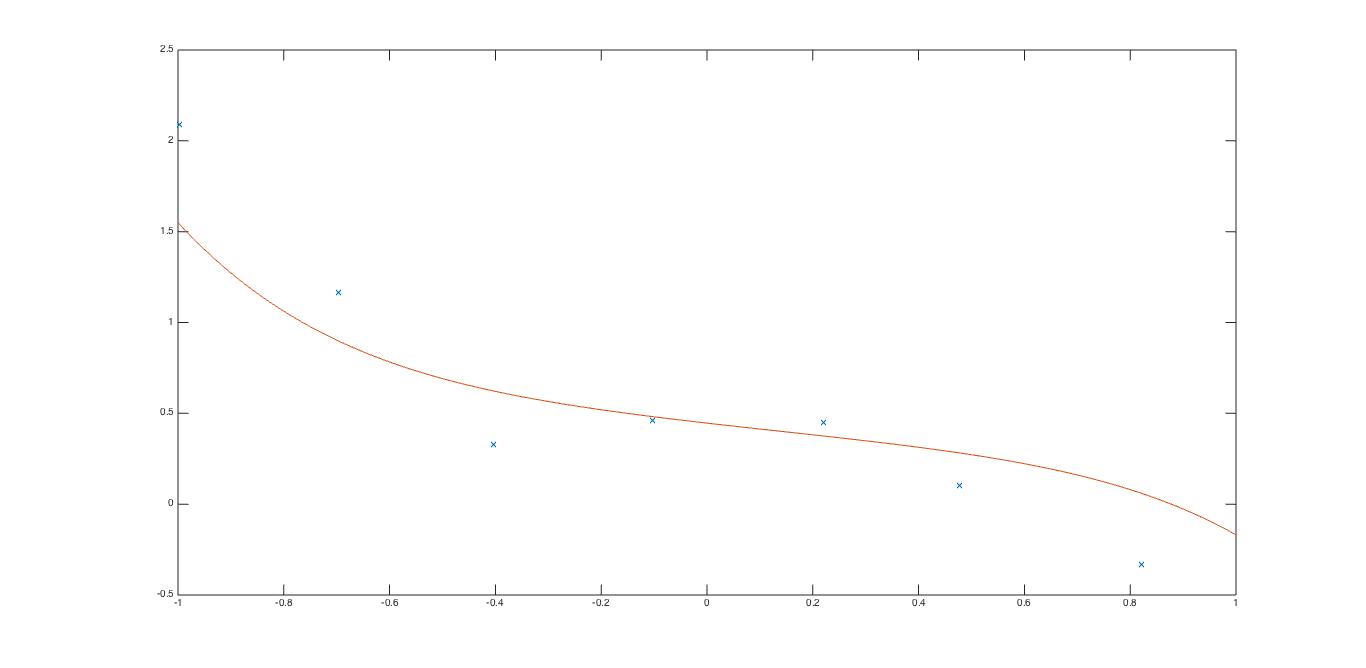
\includegraphics[width=1\textwidth]{PolynomialAlphaLambdaFunc}}
    \label{PolynomialAlphaLambdaFunc}
\end{figure}

\section{Logistic Regression}
\subsection{In the \code{logistic\_regression} folder, fill out the
    \code{sigmoid(z)} function in \code{sigmoid.m} and run
\code{plot\_sigmoid\_function.m}}
The sigmoid function was implemented as follows:\\
\begin{lstlisting}
function output=sigmoid(z)
    % Implement sigmoid function as shown in the sigmoid function formula.
    output = 1.0 ./ (1.0 + exp(1) .^ -z);
\end{lstlisting}\leavevmode \\
A plot of the output can then be seen in figure~\ref{sigmoid}
\begin{figure}
    \caption{$g(\theta^Tx)$}
    \makebox[\textwidth]{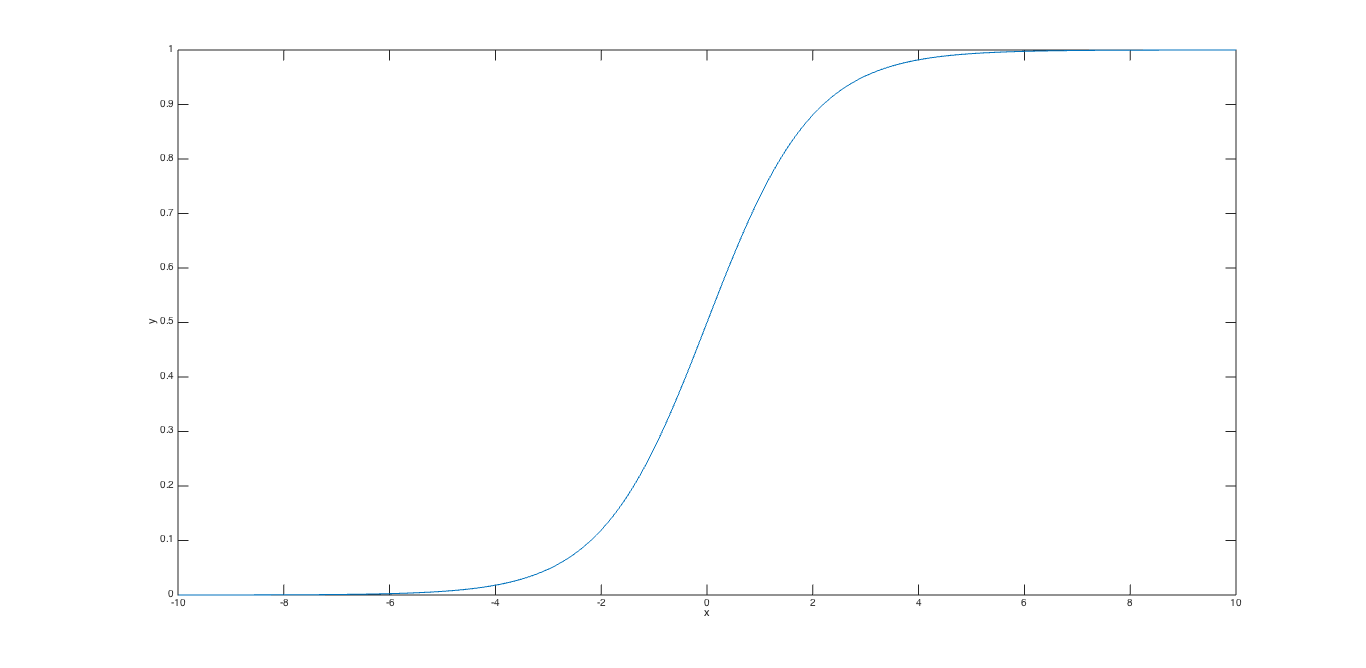
\includegraphics[width=1\textwidth]{sigmoid}}
    \label{sigmoid}
\end{figure}

\subsection{Run \code{plot\_data.m} to plot the data. Plot the data again to
see what it looks like in this new format.}
Plots of data pre-normalisation and post normalisation can be seen in
figures~\ref{LRRawData} and~\ref{LRNormalisedData}

\begin{figure}
    \caption{Data (pre-normalisation)}
    \makebox[\textwidth]{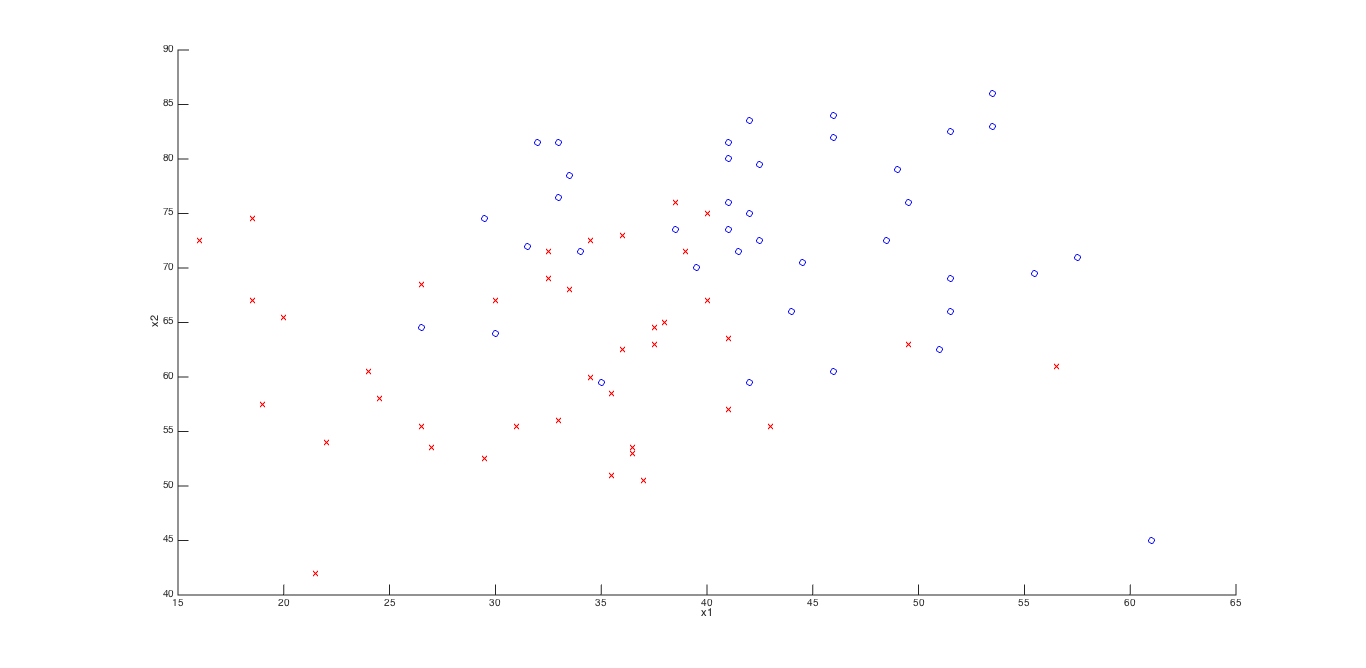
\includegraphics[width=1\textwidth]{LRRawData}}
    \label{LRRawData}
    \caption{Data (post-normalisation)}
    \makebox[\textwidth]{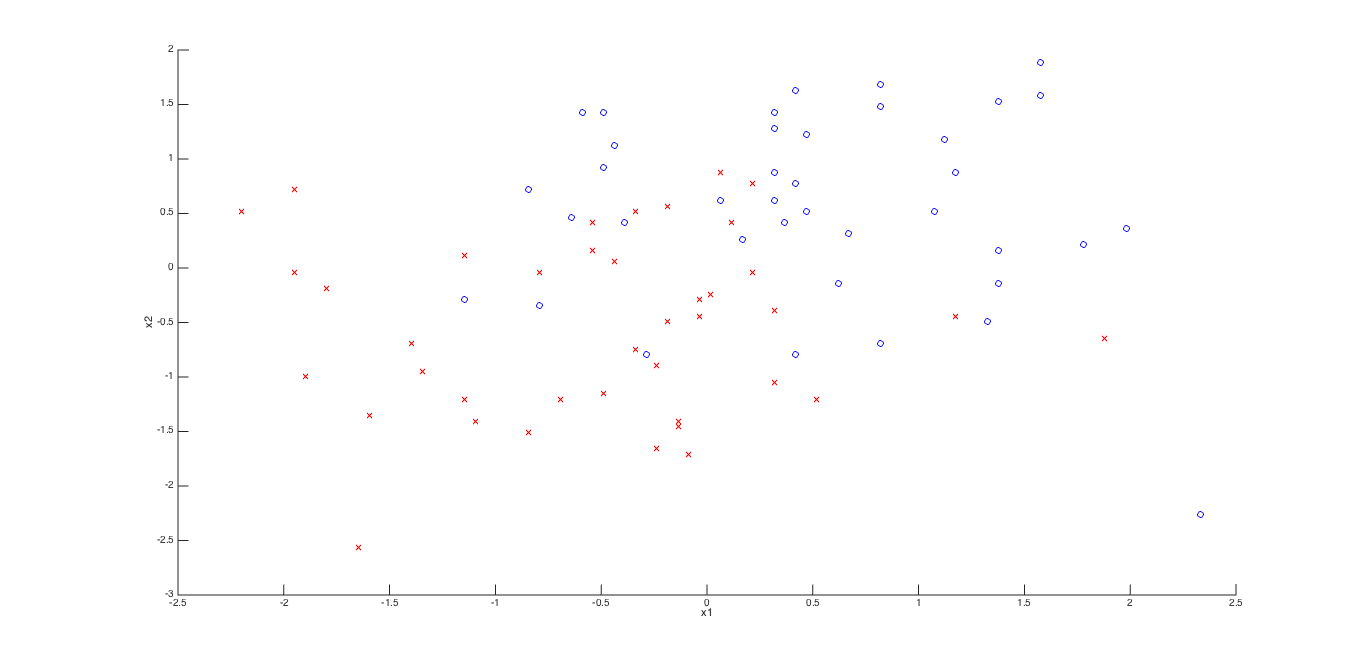
\includegraphics[width=1\textwidth]{LRNormalisedData}}
    \label{LRNormalisedData}
\end{figure}

\begin{minipage}{\linewidth}
\subsection{Modify \code{calculate\_hypothesis} so that it returns the
linear sum of the data weighted by $\theta$}
\begin{lstlisting}
function result=calculate_hypothesis(X,theta,training_example)
    % Get the value for x at the training example index provided
    x = X(training_example, 1:length(theta));

    % Calcuate the Theta weighted sum of x
    hypothesis = sum(x.*theta);

    % Apply the sigmoid function to the result
    result=sigmoid(hypothesis);
\end{lstlisting}\leavevmode \\
\end{minipage}

\subsection{Modify the line \code{cost = 0.0} in \code{compute\_cost(X, y,
theta)}...}
This section appears to already have been completed correctly prior to any
modifications. The completed code provided is as follows:

\begin{lstlisting}
function J=compute_cost(X, y, theta)
    %
    %Compute cost for linear regression. Takes an input matrix X of training
    %examples, a parameter vector, theta, and an output vector y
    %
    J = 0.0; % cost
    m = size(X,1); % no. training examples
    for i=1:m
        hypothesis = calculate_hypothesis(X,theta,i);
        output = y(i);
        cost = -output*log(hypothesis)-(1-output)*log(1-hypothesis);
        % modify this to calculate the cost function, using hypothesis and output
        %cost = 0.0;
        J =J+cost;
        
    end
    J = J*(1.0/m);
    %END OF FUNCTION
\end{lstlisting}\leavevmode \\

\subsection{What is the final cost found by the gradient descent algorithm?}
The final cost value calculate was found to be: 0.40545\\
This is illustrated in figure~\ref{LRCostEx1}

\begin{figure}
    \caption{Cost over Iterations for Logistic Regression}
    \makebox[\textwidth]{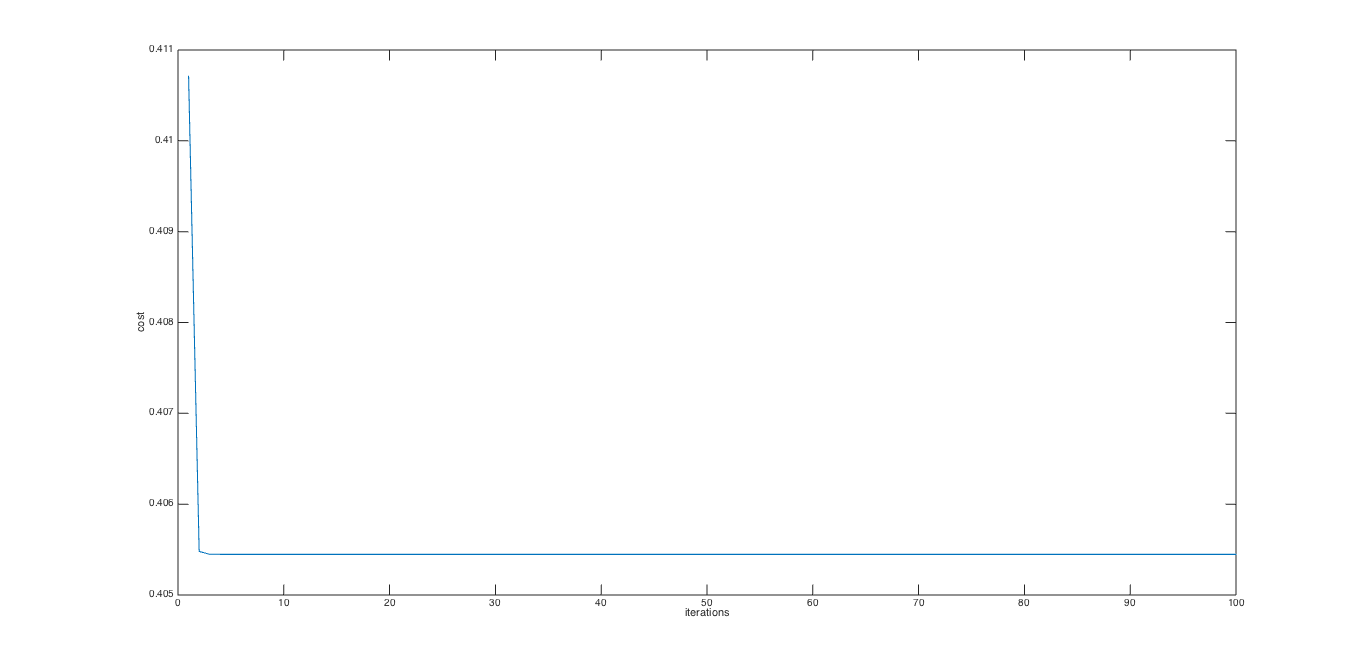
\includegraphics[width=1\textwidth]{LRCostEx1}}
    \label{LRCostEx1}
\end{figure}

\subsection{Plot the decision boundary}
The decision boundary was plotted as shown in figure~\ref{LRBoundary}

\begin{figure}
    \caption{Decision boundary}
    \makebox[\textwidth]{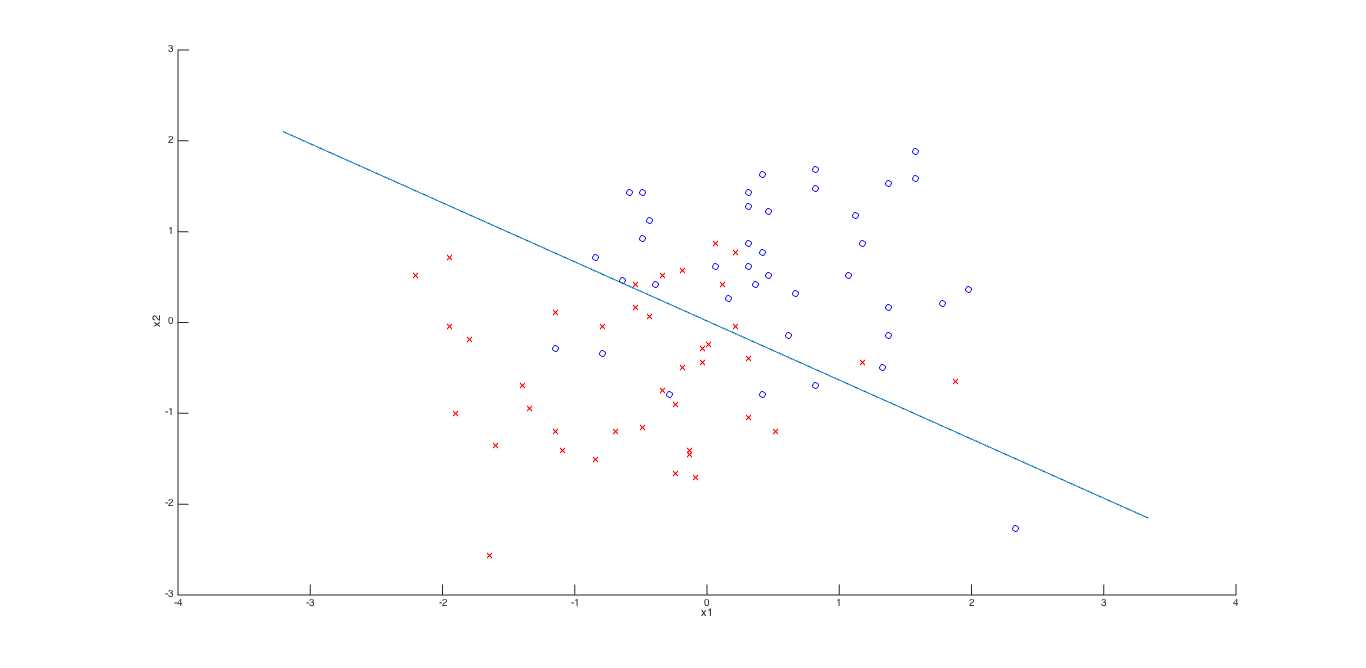
\includegraphics[width=1\textwidth]{LRBoundary}}
    \label{LRBoundary}
\end{figure}

\subsection{What is the difference between the training error and the test
    error? When does the training set generalize well? Demonstrate a split with
good and bad generalization.}
The training error is the error produced when training the model on the
training data. The test error is the error when applying the model created
using the training data to the test data.
The training set generalizes best when the set closely ressembles the test
set's shape. This produces a function that will perform well on the test set
and in theory on any new data. In this project, the best trained functions are
created from data that is spread most equally in the training set, as this
gives the best overall representation of the full dataset. This can be seen in
figures~\ref{4train} and~\ref{4test}. An example of poor generalization can be
seen in figures~\ref{6train} and~\ref{6test}.

\begin{figure}
    \caption{Function generated on training data (error: 0.20109)}
    \makebox[\textwidth]{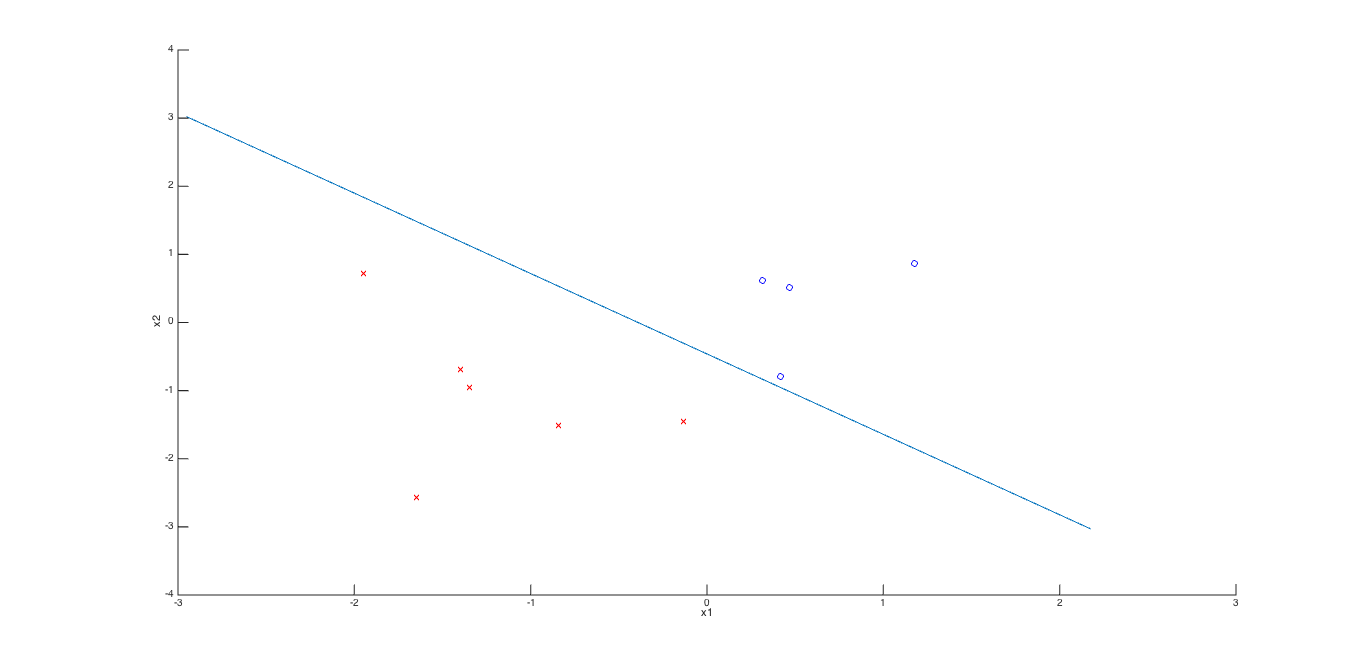
\includegraphics[width=1\textwidth]{graph4a}}
    \label{4train}
    \caption{Function plotted agains test data (error: 0.49358)}
    \makebox[\textwidth]{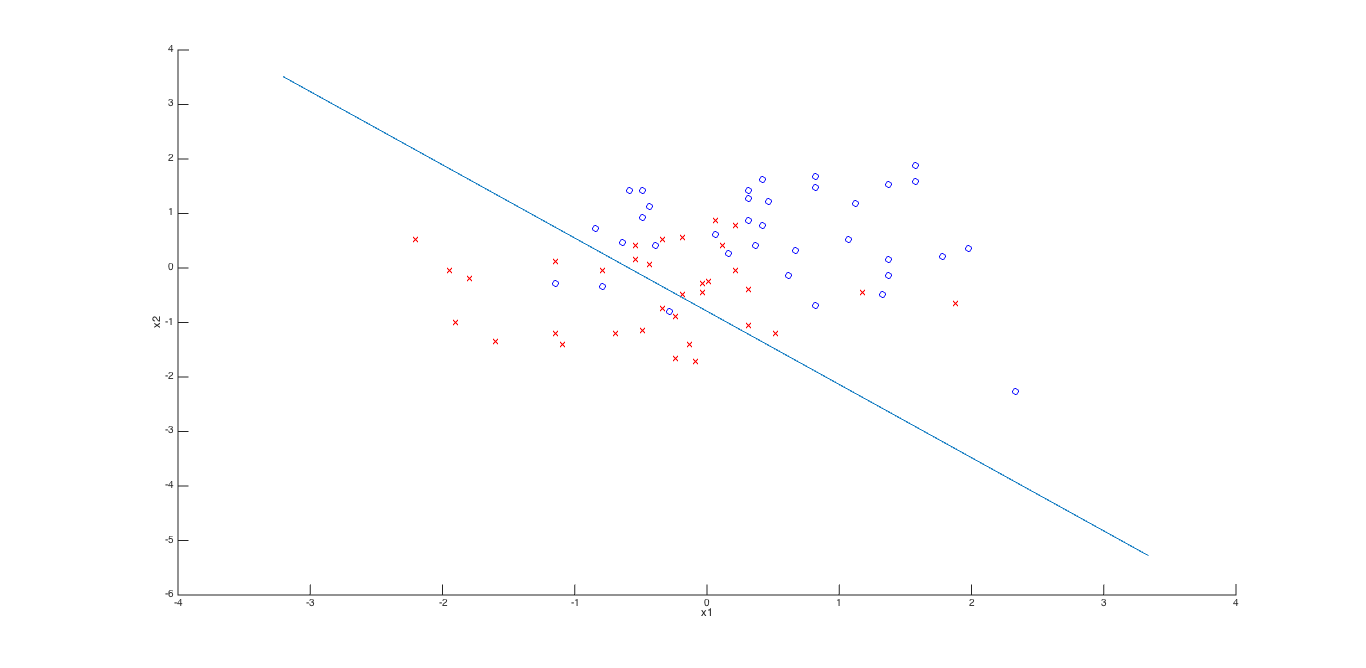
\includegraphics[width=1\textwidth]{graph4c}}
    \label{4test}
\end{figure}
\begin{figure}
    \caption{Function generated on training data (error: 0.18535)}
    \makebox[\textwidth]{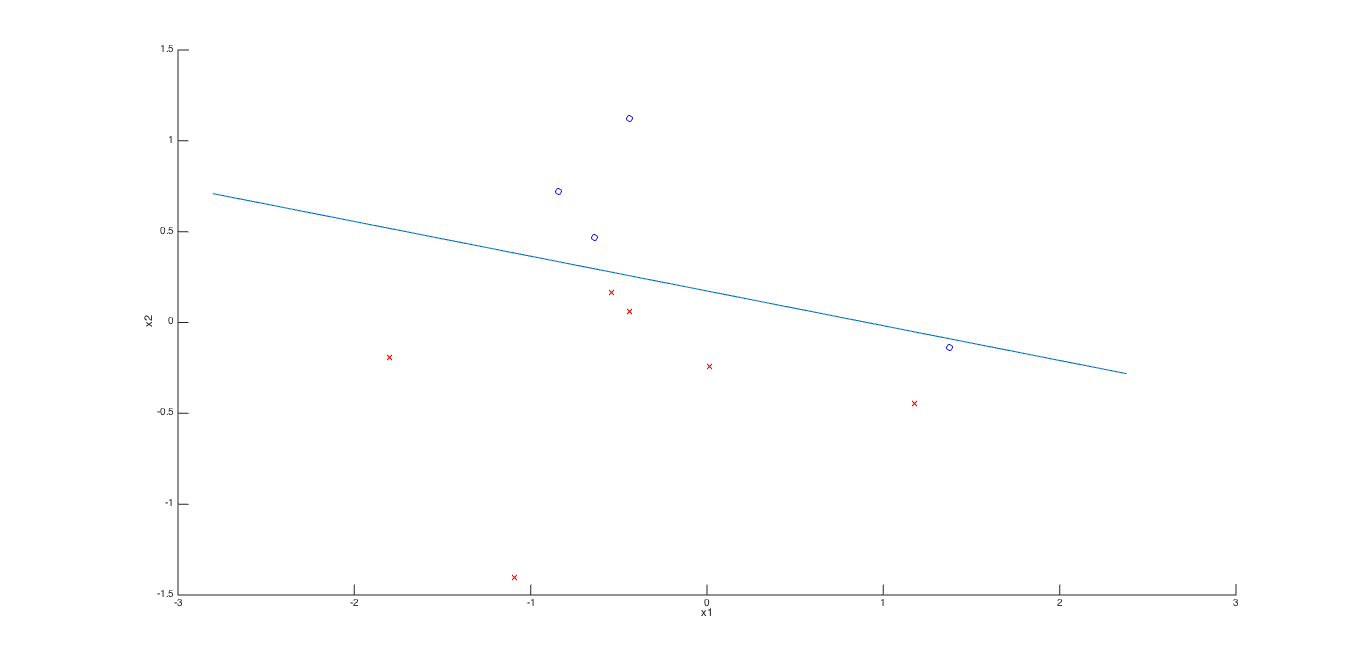
\includegraphics[width=1\textwidth]{graph6a}}
    \label{6train}
    \caption{Function plotted agains test data (error: 0.82162)}
    \makebox[\textwidth]{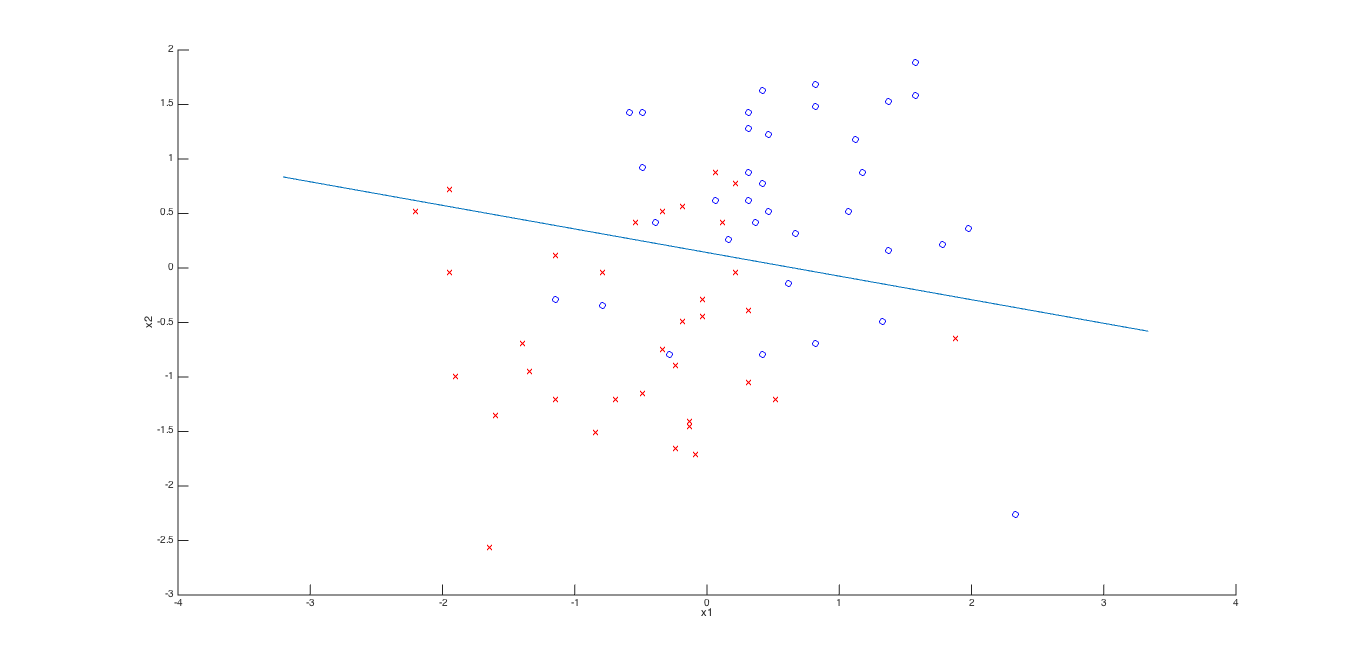
\includegraphics[width=1\textwidth]{graph6c}}
    \label{6test}
\end{figure}

\subsection{How does the error compare to using the original features}
The error using the new features is 0.39537. This is marginally lower than the
error computed using only the 2D linear features. This suggests that a
non-linear boundary may better fit the data than the linear boundary used
previously.

\subsection{Show the effect of using sets of different sizes. What does it mean
if the cost function of the training set goes down but the test set goes up?}
Graphs of training and test cost can be found in
figures~\ref{costTestTrain5},~\ref{costTestTrain10},~\ref{costTestTrain20},~\ref{costTestTrain40}
and ~\ref{costTestTrain60}.
A rise in error over iterations as the cost in training set decreases suggests
that the training set bares little resemblance to the test set. This is shown
clearly in~\ref{costTestTrain60}, where a large number of test data points
minimizes the cost over the majority of the dataset, however this does not
result in a good fit over the few remaining points used for testing.


\begin{figure}
    \caption{Training (blue)/Test (red) Error (Training: 5 data points, Test:
    75 data points)}
    \makebox[\textwidth]{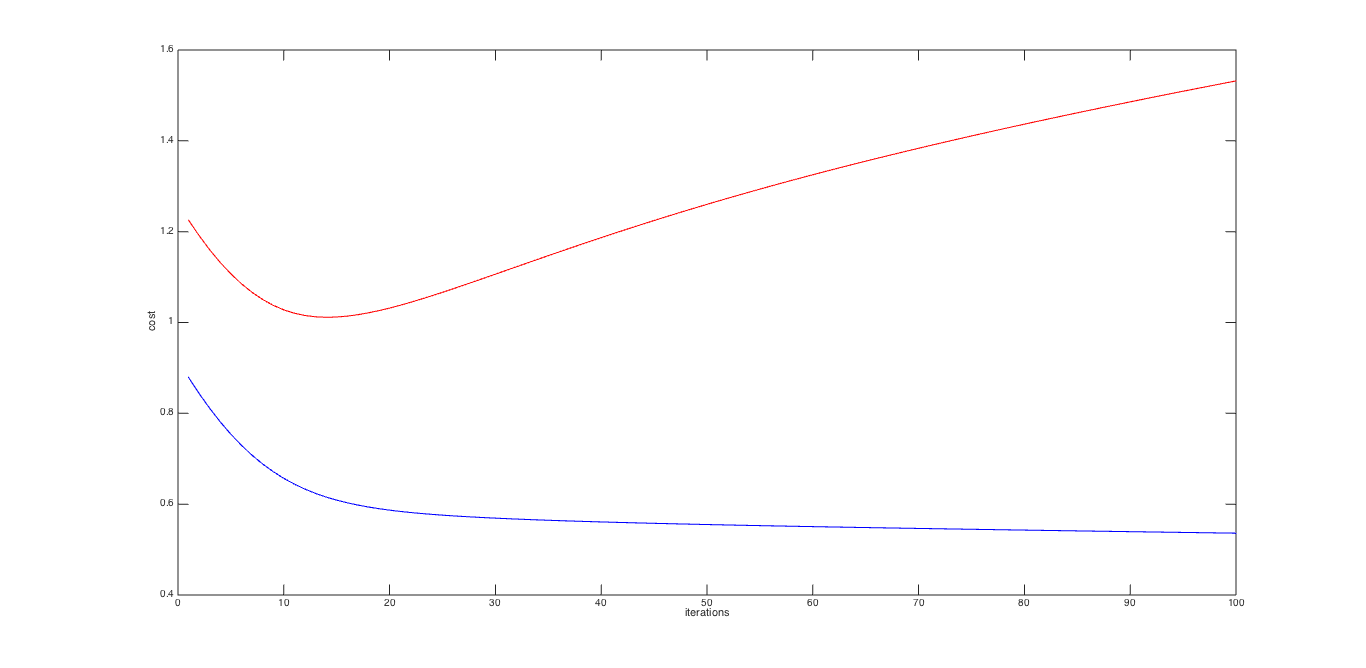
\includegraphics[width=1\textwidth]{costTestTrain5}}
    \label{costTestTrain5}
    \caption{Training (blue)/Test (red) Error (Training: 10 data points, Test:
    70 data points)}
    \makebox[\textwidth]{\includegraphics[width=1\textwidth]{costtesttrain10}}
    \label{costTestTrain10}
\end{figure}
\begin{figure}
    \caption{Training (blue)/Test (red) Error (Training: 20 data points, Test:
    60 data points)}
    \makebox[\textwidth]{\includegraphics[width=1\textwidth]{costtesttrain20}}
    \label{costTestTrain20}
    \caption{Training (blue)/Test (red) Error (Training: 40 data points, Test:
    40 data points)}
    \makebox[\textwidth]{\includegraphics[width=1\textwidth]{costtesttrain40}}
    \label{costTestTrain40}
\end{figure}
\begin{figure}
    \caption{Training (blue)/Test (red) Error (Training: 60 data points, Test:
    20 data points)}
    \makebox[\textwidth]{\includegraphics[width=1\textwidth]{costtesttrain60}}
    \label{costTestTrain60}
\end{figure}

\subsection{Explain why a logistic regression unit cannot solve the XOR
classification problem}
The XOR classification problem cannot be solved by logistic regression because
it is ``Linearly inseperable''. This is to say that it is impossible to
seperate classes in the decision space through use of a single line (as is used
in logistic regression). This can be clearly demonstrated by attempting to
seperate the two classes in figure~\ref{XOR} through use of a single line (it is not
possible)

\begin{figure}
    \caption{Example of the XOR problem}
    \makebox[\textwidth]{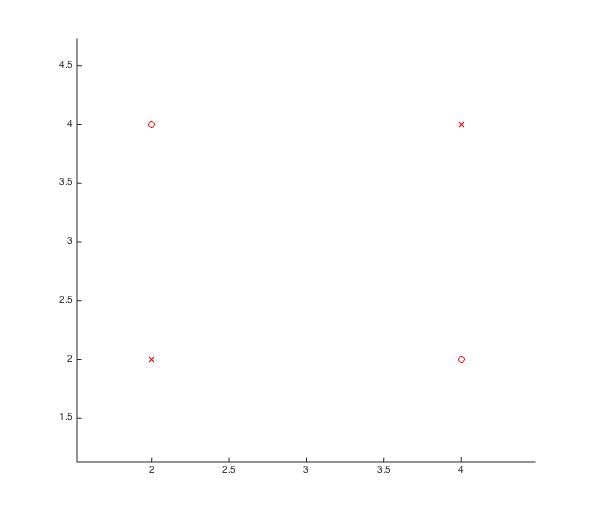
\includegraphics[width=1\textwidth]{XOR}}
    \label{XOR}
\end{figure}

\section{Neural Networks}
\subsection{Modify the sigmoid(z) function to use the sigmoid function
completed in question 1}
\begin{lstlisting}
function  sigmoid_output=sigmoid(z)
    % change this to apply the sigmoid to the data below:
    sigmoid_output = 1.0 ./ (1.0 + exp(1) .^ -z);
end
\end{lstlisting}

\subsection{Implement backproprogation}
\begin{lstlisting}[firstnumber=114]
function J=back_propagate(inputs,nn,targets,learning_rate,batch)
    %
    %Backpropagates the error and performs gradient descent on the network weights
    %
    % Step 1. Output deltas (used to change weights from hidden --> output)
    output_deltas = zeros(1,length(nn.output_neurons));
    outputs=nn.output_neurons;
    for i=1:length(outputs)
        output_deltas(i) = (outputs(i)-targets(i))*sigmoid_derivative(outputs(i));
    end
    % Step 2. Hidden deltas (used to change weights from input --> output).
    hidden_deltas = zeros(1,length(nn.hidden_neurons));
    % hint... create a for loop here to iterate over the hidden neurons and for each
    % hidden neuron create another for loop to iterate over the ouput neurons
    
    for j=1:length(nn.hidden_neurons)
        accum = 0.0;
        for k=1:length(nn.output_neurons)
           accum = accum + nn.output_weights(j,k)*output_deltas(k);
        end
        hidden_deltas(j) = nn.hidden_neurons(j)*accum;
    end

    % Step 3. update weights output --> hidden
    for i=1:length(nn.hidden_neurons)
        for j=1:length(output_deltas)
            nn.output_weights(i,j) =nn.output_weights(i,j) -(output_deltas(j) * nn.hidden_neurons(i) * learning_rate);
        end
    end

    % here we are removing the bias from the hidden neurons as there is no
    % connection to it from the layer below
    hidden_deltas = hidden_deltas(2:end);

    % Step 4. update weights input --> hidden.
    % hint, use a similar process to step 3, except iterate over the input neurons and hidden deltas

    for j=1:length(inputs)
        for k=1:length(hidden_deltas)
            nn.hidden_weights(j,k) =nn.hidden_weights(j,k) -(hidden_deltas(k) * inputs(j) * learning_rate);
        end
    end

    % this is our cost function
    J = 0.0;
    for t =1:length(targets)
        J = J + 0.5*(nn.output_neurons(t)-targets(t))^2;
    end
end
\end{lstlisting}

\subsection{What learning rate is found to be the best? What are the outputs
and error when it gets stuck in a local optima?}
The learning rate that achieved the lowest cost over several attempts was at
7.0. It achieved a cost of 7.633e-05
This resulted in output values of:
\begin{align}
h_\Theta(x) &= \begin{bmatrix}
           0.0073481 \\
           0.9882 \\
           0.98816 \\
           0.0094823
         \end{bmatrix}
\end{align}





localoptima1
cost = 0.1249
target output:0actual output0.49219
target output:1actual output0.48469
target output:1actual output0.51343
target output:0actual output0.50444

% \printbibliography
\end{document}
